\chapter{Evaluation}
\label{cha:Evaluation}

%  - result of user study, results, performance etc			
%  - describe process/use in steps with screenshots,			
%  - thoughts on development, how to make it better (recognition)			
%  - how well my initial idea worked out, what could be better			
%  -mouse clicks count (RSI)			
%  - evaluation of time using Eclipse, SR and MS SR			


After close to 400 hours spent on design and implementation, the finished prototype was created. It still does not allow to create a whole program entirely by voice, but it is ready for its first evaluation. This evaluation is not a user study per se, because it was done only by the author himself. It is therefore only an initial test of a prototype's functionality which is supposed to give an idea if the project gets closer to reaching the goal and if there is a potential worth in continuation of work. The observations arising from the test's result can also point a direction in which further development should go to, as well as it can be a foundation for a real user study that is planned in the near future.


\section{Approach}
The rationale behind the evaluation is to find out if the created system can be introduced as an alternative for the standard way of fulfilling the task of writing programs and therefore decrease the amount of mouse and keyboard usage. In order to do so, a test was carried out, the goal of which was recreation of a simple Java program using two input methods and compare the results. The two methods under test were: a common one based on typed input and cursor control, and a second one relying on voice. Because CodeSpeech is still just a prototype and not a finished product, its evaluation required partial usage of peripheral input devices in places where the necessary functionality was lacking. 

The Java program that was to be created during the test was
very simple, consisting of one interface, one abstract class implementing this interface, three classes extending the abstract one, and a main class which initialized three instances, called their methods and printed resulting text as an output to the console. All program elements can be found in Appendices \ref{appendix:soundable} - \ref{appendix:animals}, but to briefly get an idea of its complexity the class diagram is presented in Fig \ref{fig:animalDemo}. 

\begin{figure}
    \centering
    \fbox{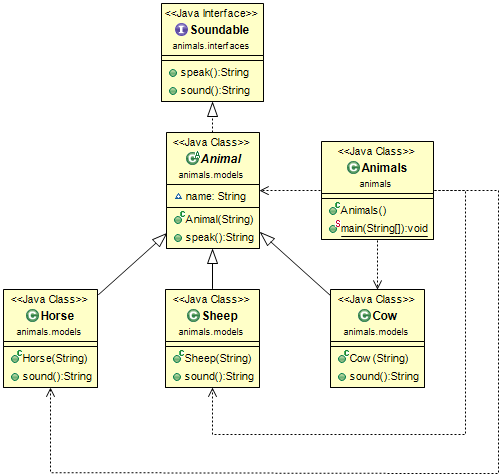
\includegraphics[width=0.9\textwidth]{images/AnimalDemo.png}}
    \caption{Class diagram of test program used to compare both input methods.}
    \label{fig:animalDemo}
\end{figure}

The workstation on which the experiment has been conducted was Lenovo Y510P laptop with Intel i7 2.40GHz processor and built in keyboard and an external optical mouse Dell DZL-MS111-L(B). The station was running Windows 10 operating system and Eclipse IDE of version 2019-06 (4.12.0). Voice recording was done by an internal microphone built into the laptop. The test was performed in English language by a non-native speaker. \\
The software tool used to record an activity of mouse and keyboard was Mousotron 12.1 \footnote{http://www.blacksunsoftware.com/mousotron.html}.
Mousotron allows to monitor different types of activities. The ones that were selected as relevant for this evaluation were:
\begin{itemize}
    \item running time,
    \item cursor distance,
    \item number of keystrokes,
    \item number of left button clicks,
    \item number of right button clicks,
    \item number of middle button clicks,
    \item number of double clicks,
    \item mouse wheel scrolls,
    \item and idle time.
\end{itemize}
Running time is measured from the beginning to the end of recording. The timer starts or stops by pressing on/off button according to the current state. Idle time measures the time in which no activity of any of the peripheral devices was detected. The delay of starting the counter was set to zero. By subtracting idle time from running time we can get the real time of keyboard and mouse usage (without distinction between them). Cursor distance monitors what distance was traveled by the cursor in either metric or English system. The distance is calculated using the size of the display and the current resolution of the screen. The display used during the test was an 18,5 inches Samsung S19A300N with resolution of 1366x768. Although this value does not give the physical distance traveled by the mouse, it still adds an important information if used in comparison between two sessions. The relation between this distance and the physical distance is proportional if the same mouse sensitivity is used. The rest of the metrics are self explanatory. Single clicks of left, right and middle button were combined to provide a single measure. The layout of the Mousotron application is presented in Fig. \ref{fig:mousotron}. 

\begin{figure}
    \centering
    \fbox{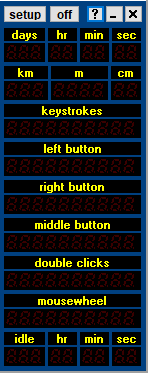
\includegraphics[width=0.2\textwidth]{images/Mousotron.png}}
    \caption{Mousotron program used to measure mouse and keyboard activity.}
    \label{fig:mousotron}
\end{figure}

In addition to input devices' metrics, another one was introduced in order to evaluate the performance of the system, namely Command Error Rate (CER). CER was measured as a ratio of the number of incorrectly interpreted (and recognized) commands (IC) versus the number of all spoken commands (N). Its formula therefore looks like this:
 $$   CER = \frac{IC}{N}. $$
 CER can be viewed as a derivative of WER of which usage did not make sense in this context. Presenting calculated WER would simply be an evaluation of speech recognition tool, and that was already done in the \textit{Tools} chapter. Instead what was preferred, was an evaluation of the performance of the whole cycle of the system, which includes interpretation, as well as recognition. The latter was made in such a way to ignore some of the words that could be in some cases accidentally introduced by SR, such as articles. Those cases should not be counted as an error if the final command was performed correctly, thus the need for CER. 
 
Once the test program was prepared and the recording software set up, the evaluation could be started. At first the program was done using the standard method, followed by the voice control method. In order for both methods to be comparable, the management of the recording had to be unified to minimize noise. The detailed description of the process backed up by screenshots can be seen in Fig. \ref{fig:steps}.
 
\begin{figure} [hbt!]
\centering\small
\begin{tabular}{@{}c@{\hspace{6mm}}c@{}} 
  \fbox{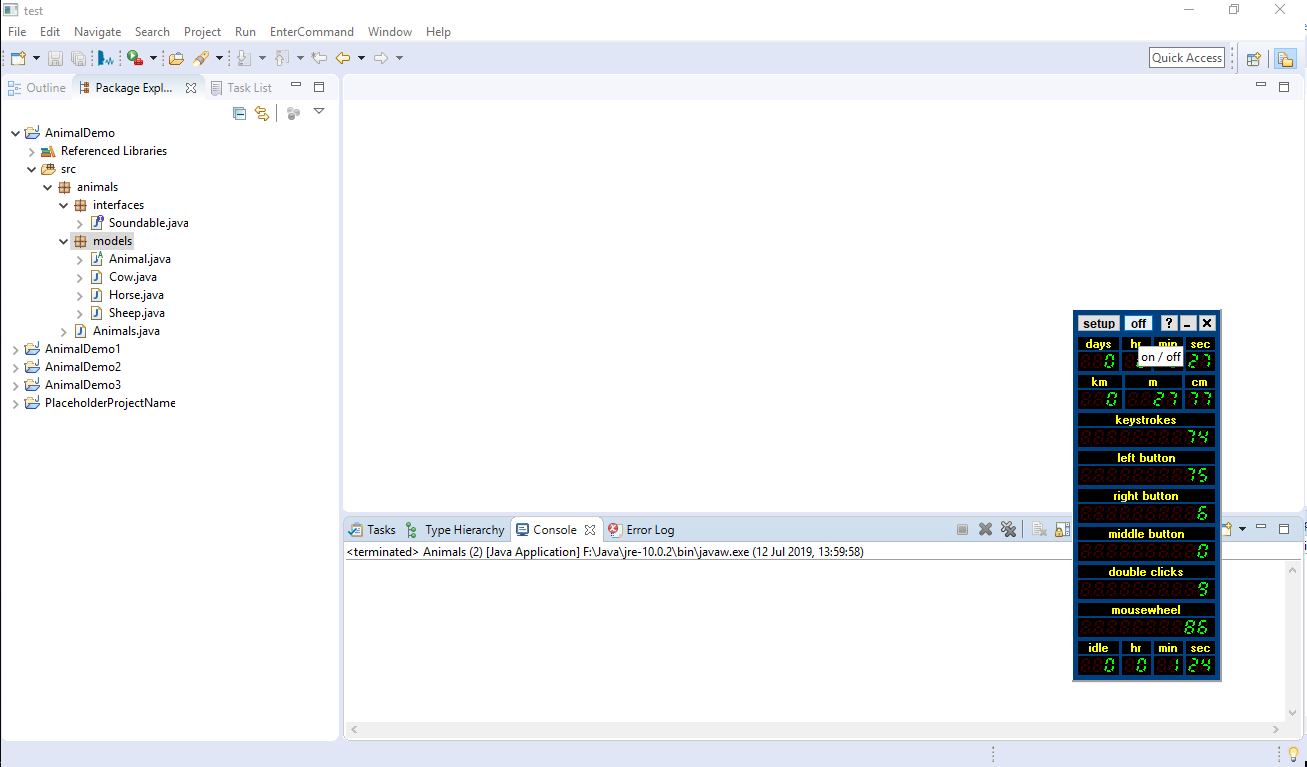
\includegraphics[width=.5\textwidth]{images/Step1.png}} &
  \fbox{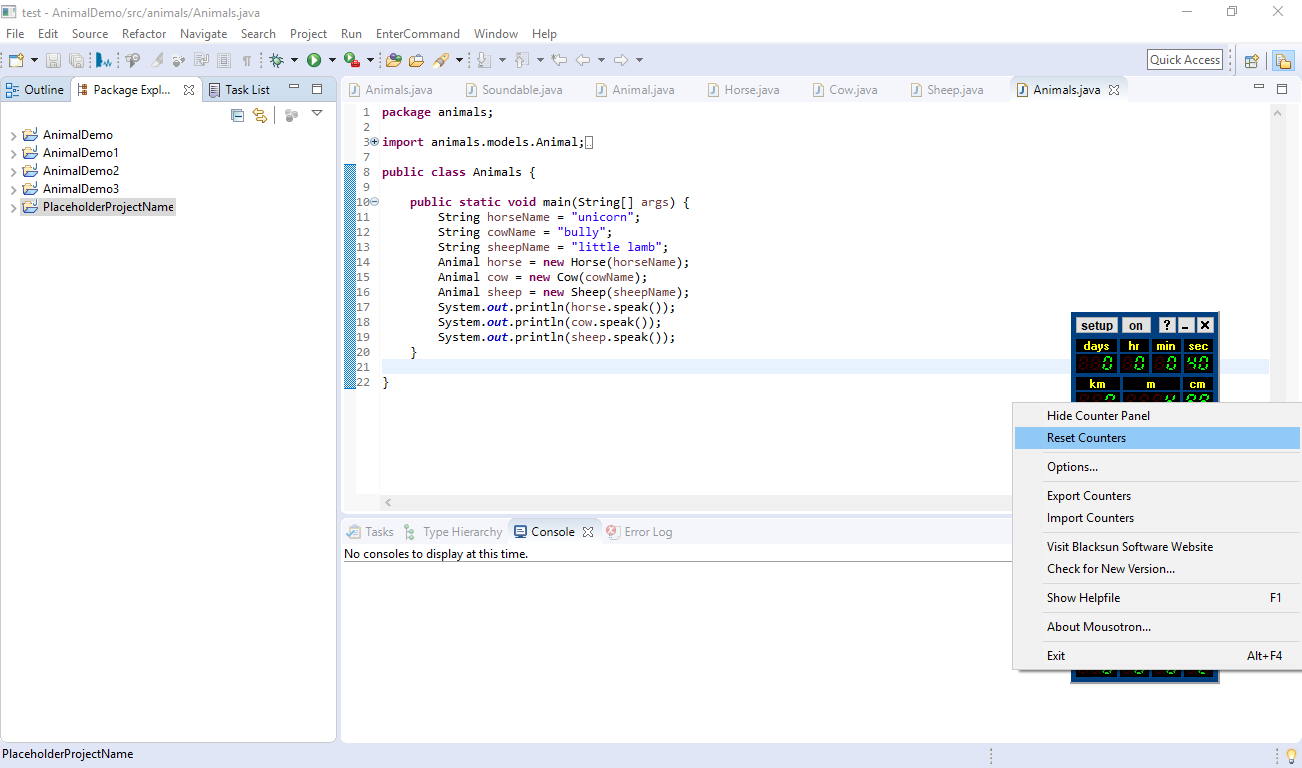
\includegraphics[width=.5\textwidth]{images/Step2.png}} 
\\
  (a) & (b)
\\[2pt]	
  \fbox{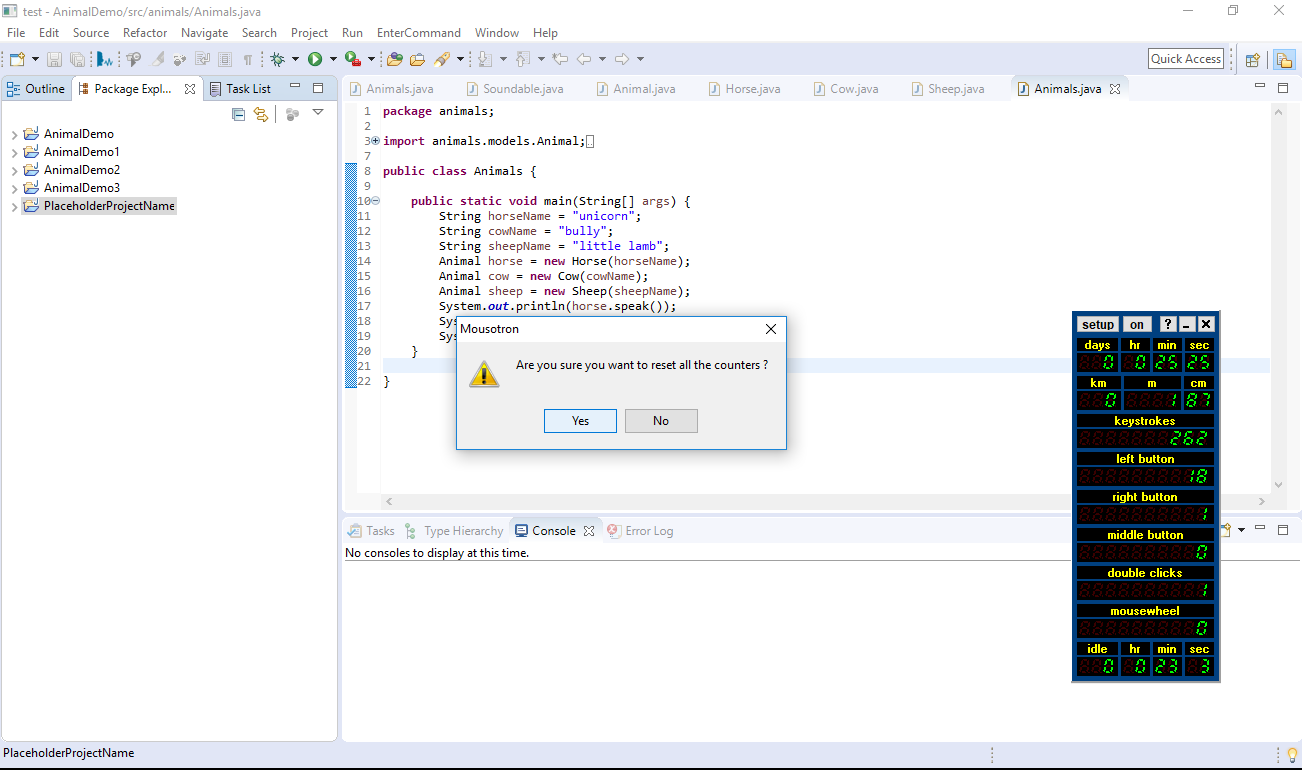
\includegraphics[width=.5\textwidth]{images/Step3.png}} &
  \fbox{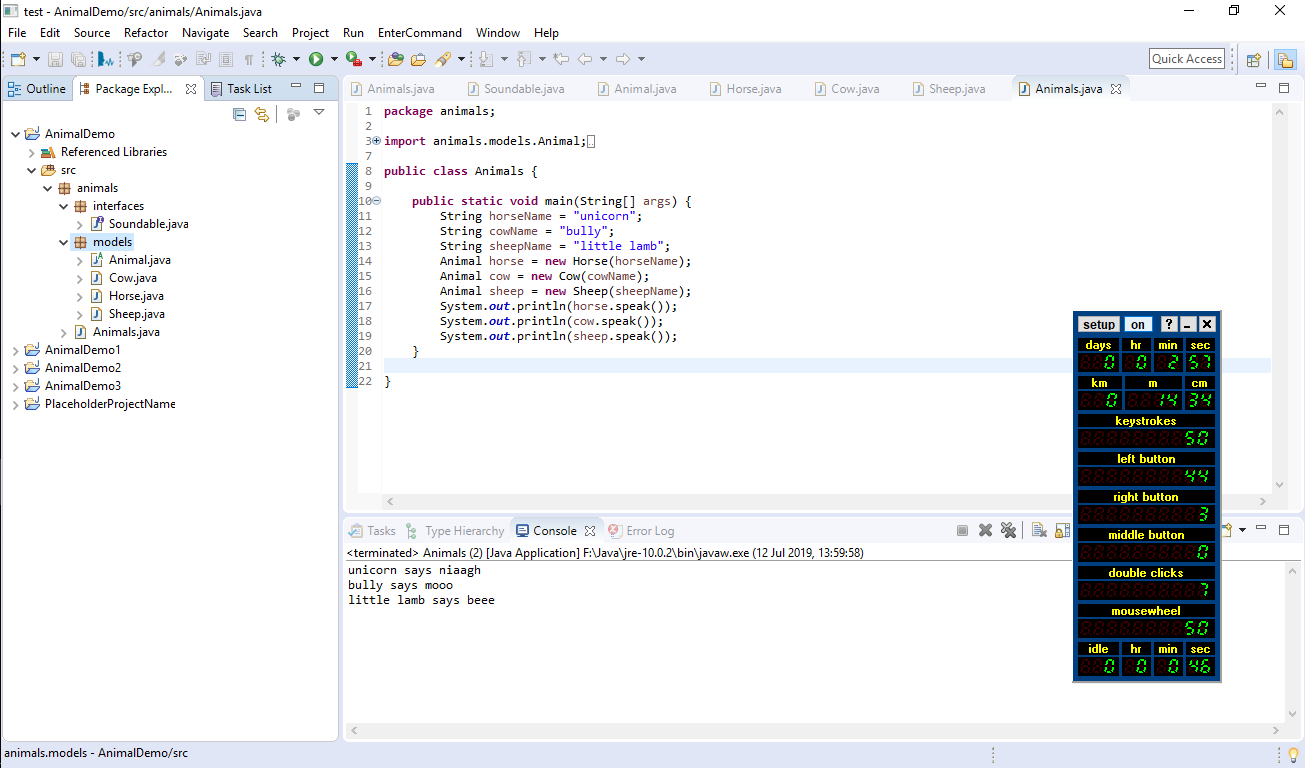
\includegraphics[width=.5\textwidth]{images/Step4.png}} 
\\
  (c) & (d)
\end{tabular}
%
\caption{ At first Mousotron and Eclipse IDE had to be both opened, visible and set to proper positions. Mousotron was set to be always on the top layer and placed in the right bottom corner of the screen to prevent covering anything considered important, to avoid the necessity of moving it during the test. This way data noise could be reduced. Once ready, the mouse and keyboard recording was started using an on/off button (a). In order to further reduce noise the counters were reset to zero via ``Reset Counters'' option (b). This made a dialog box to appear, and the counters where restarted once confirmed (c). This ensured that the initial position of the cursor was the same for both methods. After confirmation programming could begun. Finish was marked by the successful run of the program with the correct output printed into console. To stop recording, the on/off button had to be pressed again (d).}
\label{fig:steps}
\end{figure}
 
\section{Results}

The results of the evaluation of two different input methods are presented in Tab. \ref{tab:results}. In the table one can see the scores of previously selected measures. The first column titled as ``Method 1'' represents the standard way of providing input through mouse and keyboard, while the programming done mainly by voice with a support of standard input devices is titled ``Method 2''. 
As it comes to CER, the final score was 0,295 (~30\%) with a number of incorrectly interpreted commands being 67 and the total number of spoken commands was 227. 

\begin{table}
    \caption{Results of evaluation.}
    \label{tab:results}
    \centering
    \setlength{\textwidth}{5mm} % separator between columns
    \def\arraystretch{1.25} % vertical stretch factor
    \begin{tabular}{|r||c|c|}
        \hline
        & \emph{Method 1} & \emph{Method 2} \\
        \hline
        \hline
        Total time & 5 min 57 s & 24 min 54 s \\
        \hline
        Device usage time &  5 min 06 s & 1 min 55 s\\
        \hline
        Cursor distance & 887 cm & 154 cm \\
        \hline
        No. of keystrokes & 876 & 262 \\
        \hline
        No. of clicks &  84 & 17  \\
        \hline
        No. of double clicks &  19 & 1\\
        \hline
        Mouse wheel scrolls &  0 & 0\\
        \hline
    \end{tabular}
\end{table}

\section{Discussion}

The discussion about the results has been divided into three sections, focusing on different aspects: programming time, interaction with mouse and keyboard and CER. The results show that the time needed to complete a program via voice input is indeed longer, nonetheless it requires less interaction with input devices. The number of incorrect commands was relatively small, however, there is still a lot of room for improvement. More details can be read below.

\subsection{Programming time}

As it can be seen, completion of the test using Method 1 took only 5 minutes and 57 seconds, while Method 2 needed 24 minutes and 54 seconds. This in fact means that programming using CodeSpeech is around four times slower. That is a significant difference and it proves that CodeSpeech is not suitable to replace the standard method just yet. It is assumed that there are several reasons that make standard way faster. The first could be many of the options built-into IDE that speed up programming experience, such as auto-completion of text, keyboard shortcuts, problem solving suggestions, creation wizards and others. The second reason that can accelerate writing code is possibility of copying specific structures and refactoring them instead of typing them from the very beginning every time. Third reason that is suspected to have a relevance is error correction. Speech recognition systems, when recognized correctly do not introduce typos as it happens when typing. However, when recognition is not correct, trying to fix it might take longer than correcting a typo, especially when the result of recognition happens to be false more than once. Couple of times during the test a situation occurred, where one command had to be given many times over. The worst situation that has happened was in experimental free speech mode, when incorrect text was entered and the command to reverse last change was also falsely recognized. That resulted in appending incorrect text to the previous one rather than correcting an error. Now the reverse operation had to be done twice, and it could again be falsely recognized and so on. Finally, the author, who performed the test has over 5 years experience in programming, and even more in interacting with a computer using a mouse and keyboard while programming by voice is a new concept. Lots of mistakes were made, such as saying an incorrect command, stopping in the middle of the utterance to think about what comes next and forgetting about going back from free speech mode. 

\subsection{Interaction with mouse and keyboard}
Although the time required to finish the program was longer in case of Method 2, the time of mouse and keyboard usage was shorter by 3 minutes 11 seconds decreasing it to 37,6\%. Distance traveled by the cursor was shortened to 17,4\%. Method 2 required 614 less keystrokes (29,9\%) and the number of clicks and double clicks was decreased to 20\% and 5\% respectively. Mouse wheel was not used at all during the test. \\
It is clear that the usage of mouse and keyboard has been decreased quite substantially in programming by voice approach. One might argue that despite that, the increase of time needed to complete a simple program is not worth the change. The author of the thesis himself agrees with that statement, however, it is worth to remind that these are the results of the initial test and the system under evaluation is still a prototype. With the enhancement of the project and increase in functionality, usability and with better error correction a day might come when the tool becomes competitive in performance while keeping its benefits of limiting mouse and keyboard use. 

\subsection{CER}
The performance of the system could be improved by decreasing CER, on which two factors have an impact, namely accuracy of speech recognition and strictness of interpretation based on grammar. Obviously, the better the recognition, the easier is to match the grammar, however it cannot be assumed that SR will always give perfect results, that is why handling it properly by interpreter should allow some flexibility to make up for mistakes done by SR. Improving both factors will result in smaller amount of needed repetitions an error corrections and and thus, shorter time of programming. In the meantime, the next section presents some ideas about how to possibly improve the system.


\section{Ideas for improvement}
During the evaluation a couple of different ideas of how to make the program better came up. In this section some of them are presented. At the beginning the focus of the discussion is on the ideas how to make recognition better as it is obviously one of the most important factors. This at times intertwines with the ideas for improvement of interpretation. Later the section pivots to discuss how to improve usability, and finally gives examples of features that increase performance of the system.

\subsection{Interpretation of more propositions}
Speech recognition systems solve classification problem. The results that are provided are based on probability. Many SR toolkits give the whole list of potential solutions, and it is not different in the case of Google API. The output returned by the API is a list of phrases, ordered by measure of confidence. It might happen, that the correct phrase is not on the surface but rather is somewhere deeper in the list. In the current version, CodeSpeech trustfully takes the top item and do not care about the others. Perhaps interpretation could be done on all of the propositions until a correct one is found? This of course could slow down the whole cycle, unless interpretation on different phrases is done in parallel. \\
An alternative to this approach is to add an additional feature, which would allow the user to iterate through the list of propositions, \eg by running the command ``try next''. Therefore every correct recognition done at the first try would not slow down the system, and in case of incorrect one the user would have control.

\subsection{Context recognition}
Another idea focuses on adding context to the process of recognition. Google Cloud Speech-to-Text is good in recognizing continuous speech, but that does not ensure correct results in systems with limited amount of words or phrases. Programming languages themselves have restricted list of keywords. It comes to mind, that a smart idea would be to provide some context in order to increase performance and omit cases in which the phrase like ``change return type...'' is being recognized as ``Chun's restaurant...'', which of course in the programming world does not make any sense (unless Chun's restaurant is supposed to be used as a variable name). Since in CodeSpeech interpretation of recognized phrase is based on grammar, why not to use it as a context for recognition as well?  Google API does not supply such an option, but CMUSphinx tools do. The grammar it is using is different from the one used by ANTLR, so its counterpart in the form of Java Speech Grammar Format (JSGF) would need to be created. That obviously comes with some consequences, namely whenever a change is to be introduced to the grammar, both files have to be modified accordingly. Perhaps this process could be automated.  

Next concept of context based recognition relies on the third option provided by CMUSphinx, which is keyphrase recognition. Once a text file with specified phrases is created, it can then be used to trigger an action on a recognized keyphrase or single keyword ignoring the rest. That seems like a better solution in comparison to grammar, because grammar tend to be very strict, and if at least one unexpected word (such as an article) appears in the middle of a sentence, the match is not found. That makes keyphrase approach more flexible. It does sound promising, however, how it will work in practice must be investigated. 

It may be that combining one of the aforementioned approaches (or both) with continuous, free speech recognition can give even better results. CMUSphinx allows for changing between modes during run time. That could require modifying the way voice commands are given to consist of phases. Initially, the SR is set up to keyphrase detection. Once the keyphrase has been detected the mode is switched to listening for continuous speech (when the name is to be spoken), and then back. An example of recognition divided into phases could look like this:
\begin{enumerate}
    \item command ``create new public method named'' is given,
    \item keyphrase is detected, and the mode switches to free speech listening,
    \item when the user is notified, ``get current state'' name is spoken,
    \item operation creating new method of name ``getCurrentState'' is created and the mode switches back to keyphrase recognition.
\end{enumerate}
This way seems like it could again slow down the whole process a bit, but perhaps if the outcome will mean more accurate recognition, thus a decrease in the amount of repetitions needed, in the end it might turn out to actually be faster.
In order to easier operate with names that already exist in the project, perhaps a good idea is to dynamically store them in the form of separate keyphrase file. This way at the beginning of name giving phase, the recognition could be performed in keyphrase mode (just the file is changed to the one consisting of names). If relatively strong match is found, the name will be brought up, but if not then probably a new name is being given, so recognition proceeds in continuous mode. This approach could increase precision and maybe decrease error rate in code reuse.

\subsection{Combining recognition systems}
In previous subsections the usage of CMUSphinx was considered to be applied in potential future improvement work, despite the fact that in the previous sections thi technology was rejected for not being good enough. It is true that CMUSphinx's default models do not ensure a good recognition for non-native speakers. Even recommended acoustic adaptation did not provide enough improvement (would require much more adaptation than it has been done). It comes, however, with the tools to build completely new acoustic and language models based on a phonetic dictionary, which can be modified according to needs. Perhaps CMUSphinx will never be as good in continuous recognition as its commercial counterpart belonging to Google, nonetheless, it might prove good enough for the recognition of limited list of commands/words if the models are being built specifically for this purpose. Therefore the recognition of commands could be left to CMUSphinx in its more suitable modes mentioned earlier, while continuous recognition used \eg for names could be left to Google Cloud Speech-to-Text or yet another tool. The process of building all models from scratch is going to be time consuming and will require a lot of work, but it may be worth considering anyway. 

\subsection{Better error correction}
For now the only means of error correction works for the text editor, where source code is written. By saying ``undo last'' the last change in the text is reversed. In some situations, however, it might be necessary to perform reverse action more than once. In cases like this the command ``undo last'' needs to be spoken repeated couple of times. It gets even worse when this command is falsely classified and an extra text is entered. That adds to the stack of needed corrections. To make it better, it should be possible to give a number of times the reverse operation has to be made, for example ``undo last three times''. That could speed up the process. \\
Additionally other means of error correction should be implemented, such as a possibility to change the wrong name, move a structure and basically to provide more options of manipulation, as well as allowing to use some of the IDE's proposed solutions in an easy way. This should be done not only for the text editor, but also for other elements, such as package explorer. 

In SR tools such as Windows Speech Recognition, when the users are not satisfied with the inserted word, they can give a command ``correct' and are then presented with a list of options that can be selected by saying a number of a line with correct phrase. Borrowing from that a similar list could be made available to the user when an incorrect operation was performed or when it is not clear what the user is trying to do. Perhaps this solution could also be used for future reference and help the system learn to avoid similar mistakes in the future. 

\subsection{Adaptation}
Previous subsections inspired another idea. Some speech recognition systems allow for adaptation of the model with the recordings of the users to improve the results. Adding this as a feature could make sure that CodeSpeech achieves the same performance when working in different environments, voices, accents once it learns from those recordings. Whenever the users are not satisfied with the results they can start teaching mode in which they will have to read out loud a couple of sentences or perhaps specific commands. The process can be repeated a couple of times and with each improvement should be visible.

\subsection{Feedback}
Until now the focus was put on recognition, interpretation and operation execution, to make sure the system works. Currently there exists no feedback system built into the plugin, which makes it difficult to use. Whenever an error occurs or an exception is thrown, the user is not notified about that fact and therefore is unaware of why no action was performed or what he/she did wrong. Even if no error occurred, but simply the recognition was incorrect and nothing happens the user does not know the reason for it. A way to give back information of the current status should be implemented. Feedback system could be a text window (similar to the console) that displays either the recognized text, some details about performed action (if any) or simply an information that the system did not understand or wrong action was undertaken. 

\subsection{Improve voice control experience}
Ideally, the end product's input is going to be flexible enough to invoke one operation with different sentences that have the same meaning in English. If this goal turns out to be hard to reach, maybe it can be worth to consider giving the users the possibility to define their own commands for each action. All keywords could be presented in table form in which respective words could be overwritten. After the modification the program reacts to different phrases.
Despite which option will end up being in the finished product, it should be possible at any time for the user to open a list of phrases that are available in the current context. Even the author had to go back to the grammar file in order to check the proper way of saying a specific phrase. 

Another observation made during the test was that whenever a break was made in the middle of the recognition \eg between words or to think about the proper name, the sentence was broken in half and whatever has been said until this point was sent to recognition. That enforces on user to think first about what is to be said and then say it without a pause. That does not seem very convenient. A better approach would be to save the state of the current command wherever it was broken. This could be achieved by introducing more listeners (perhaps each for each state) and replace the current one with the new one every time a keyword is recognized. The context is passed in between the listeners anyway, so no information would be lost. When the users find themselves in the middle of the command which they do not want to finish, they could simply go back to the initial state by saying ``cancel''. The current implementation surely allows for such a solution.

\subsection{More features}
The amount of features available in CodeSpeech is very limited. There are plenty of structures that cannot be created, modification possibilities are almost not existing and there are lots of options that IDE provide that are not accessible via CodeSpeech. The base of the system is more or less finished and it can be easily extended to provide new functionalities. However, adding new options takes time and so bringing the project to truly satisfying state will require large amounts of work.\\
With more options added the usability of the project would of course increase. Some examples of features to be implemented are:
\begin{itemize}
    \item{better editor navigation,}
    \item{text editing similar to this available in SR tools,}
    \item{possibility to select, copy and paste parts of code, project elements or AST nodes,}
    \item{possibility to call IDE commands such as indent of the code, performing a quick fix action, auto import of libraries \etc}
\end{itemize}

